\documentclass[12pt,english]{article}
\usepackage{mathpazo}
\renewcommand{\familydefault}{\rmdefault}
\usepackage[T1]{fontenc}
\usepackage[latin9]{inputenc}
\usepackage{geometry}
\geometry{verbose,tmargin=1in,bmargin=1in,lmargin=1in,rmargin=1in}
\usepackage{color}
\usepackage[dvipsnames]{xcolor}
\definecolor{oucrimson}{RGB}{132.,22.,23.}
\usepackage{babel}
\usepackage{booktabs}
\usepackage[authoryear]{natbib}

% Useful Packages
%\usepackage{bookmark} % For speedier bookmarks
\usepackage{amsthm}   % For detailed theorems
\usepackage{amssymb}  % For fancy math symbols
\usepackage{amsmath}  % For awesome equations/equation arrays
\usepackage{array}    % For tubular tables
\usepackage{longtable}% For long tables
\usepackage[flushleft]{threeparttable} % For three-part tables
\usepackage{multicol} % For multi-column cells
\usepackage{graphicx} % For shiny pictures
\usepackage{subfig}   % For sub-shiny pictures
\usepackage{enumerate}% For cusomtizable lists
\usepackage{pstricks,pst-node,pst-tree,pst-plot} % For trees

\usepackage[unicode=true,pdfusetitle,bookmarks=true,bookmarksnumbered=false,bookmarksopen=false,breaklinks=true,pdfborder={0 0 0},pdfborderstyle={},backref=false,colorlinks=true]{hyperref}
\hypersetup{citecolor=oucrimson,filecolor=oucrimson,linkcolor=oucrimson,urlcolor=oucrimson}
\usepackage{breakurl}

\begin{document}

\title{Introduction to Optimization}
\author{Econ 5253: Data Science for Economists\\ Prof. Tyler Ransom\\ University of Oklahoma}
\date{Spring 2020}
\maketitle

\section{What is ``optimization''?}

The word ``optimization'' generally means ``the action of making the best or most effective use of a situation or resource'' (Google's dictionary). In data science, this could refer to two different things:
\begin{enumerate}
    \item Streamlining some sort of automated process
    \begin{enumerate}
        \item e.g. ``We \emph{optimized} the web scraping script so that it now runs in half the time and has 40\% fewer lines of code.''
    \end{enumerate}
    \item Finding the optimum of an objective function (or ``selecting the best element from some set of available alternatives,'' according to Wikipedia)
    \begin{enumerate}
        \item e.g. ``Our preferred model estimate is the set of parameters that \emph{optimizes} the sum of the squared distance between the data and the model.'' {[}in this case, ``optimize'' would mean ``minimize''{]}
    \end{enumerate}
\end{enumerate}
The \textbf{second} of these two definitions is what you should think of when you hear ``optimization'' in a data science context.

\section{Ways to optimize}
There are many different ways we can optimize a particular objective function. The two most common ways---which we will discuss today---are known as \textbf{minimum distance estimation} and \textbf{maximum likelihood estimation}. These are two different but related ways of expressing the objective function.

In any optimization problem, the data scientist must also choose an \emph{algorithm} with which to optimize, if the optimum cannot be expressed in a math formula. The three most popular optimization algorithms are:
\begin{enumerate}
    \item gradient descent
    \item stochastic gradient descent
    \item L-BFGS
\end{enumerate}
We'll talk about these algorithms a bit later in the course.

\section{Math: the classical linear model}

Let's suppose we have the classical linear model:

\begin{equation}
y_{i}=x_{i}^{\prime}\beta+\varepsilon_{i}\label{eq:1}
\end{equation}
where $y_{i}$ is the outcome for observation (equiv. training example) $i$, $x_{i}$ are the covariates (equiv. features) of observation $i$, $\beta$ are parameters to be estimated, and $\varepsilon_{i}$ is the error term.

We can rewrite (\ref{eq:1}) in vector form:
\begin{equation}
y=X\beta+\varepsilon\label{eq:2}
\end{equation}
where now $y$ is a vector (i.e. column of data), $X$ is a matrix (i.e. a table of data), $\beta$ are exactly the same as before, and $\varepsilon$ is an (unobservable) error term vector. 

\subsection{Optimization method 1: least squares}

We can define our objective function so that we minimize the (squared) distance between $X\beta$ and $y$. In this sense, minimizing the distance will give us the best fit (i.e. optimum) of the model given the data. In formal terms, we want to
\begin{align}
 & \min_{\beta}\sum_{i}\left(y_{i}-x_{i}^{\prime}\beta\right)^{2}\nonumber \\
= & \min_{\beta}\sum_{i}\varepsilon_{i}^{2}\nonumber \\
= & \min_{\beta}\varepsilon^{\prime}\varepsilon\label{eq:3}\\
= & \min_{\beta}\left(y-X\beta\right)^{\prime}\left(y-X\beta\right)\nonumber 
\end{align}
Note that the four equations above are all equivalent. We can conserve on notation by utilizing vector and matrix notation (e.g. $\varepsilon^{\prime}\varepsilon$ is the dot product of the $\varepsilon$ vector with itself).\footnote{A related objective function to the one above is to minimize the \emph{absolute value} of the distance between $y$ and $X\beta$. This model is known as \emph{least absolute deviations} and the parameter estimates at the optimum correspond to the \emph{median regression} model rather than the OLS regression model (the linear prediction of which passes through the mean).}

\subsubsection{Using calculus to solve for the least squares estimator}

We can solve this optimization problem using calculus:

\begin{align*}
 & \min_{\beta}\left(y-X\beta\right)^{\prime}\left(y-X\beta\right)\\
    = & \min_{\beta}\left(y^{\prime}y-\beta^{\prime}X^{\prime}y-y^{\prime}X\beta+\beta^{\prime}X^{\prime}X\beta\right)
\end{align*}
How do we use calculus to find an optimum? Take first-order conditions and set them equal to zero:
\begin{align}
\left[\beta\right]: & -\frac{\partial}{\partial\beta}\beta^{\prime}X^{\prime}y-\frac{\partial}{\partial\beta}y^{\prime}X\beta+\frac{\partial}{\partial\beta}\beta^{\prime}X^{\prime}X\beta\label{eq:4}\\
0= & -X^{\prime}y-X^{\prime}y+2\left(X^{\prime}X\right)\hat{\beta}\nonumber \\
0= & -2X^{\prime}y+2\left(X^{\prime}X\right)\hat{\beta}\nonumber \\
X^{\prime}y= & \left(X^{\prime}X\right)\hat{\beta}\nonumber \\
\hat{\beta}= & \left(X^{\prime}X\right)^{-1}X^{\prime}y\nonumber 
\end{align}
which is known as the \emph{OLS estimator}.

\subsubsection{Checking second-order conditions}

How do we know if our optimum is a minimum or a maximum? We need to check that the second-order conditions are satisfied. For a \emph{minimum}, we need the second derivative to be \emph{positive}. Taking the derivative of our first-order condition with respect to beta, we get:
\begin{align}
0 & <\frac{\partial^{2}}{\partial\beta\partial\beta^{\prime}}\left(y-X\beta\right)^{\prime}\left(y-X\beta\right)\label{eq:5}\\
0 & <\frac{\partial}{\partial\beta^{\prime}}\left[-X^{\prime}y-X^{\prime}y+2\left(X^{\prime}X\right)\hat{\beta}\right]\nonumber \\
0 & <2\left(X^{\prime}X\right)\nonumber \\
\left(X^{\prime}X\right) & >0\nonumber 
\end{align}
This condition is satisfied so long as the following conditions hold:
\begin{enumerate}
\item $X$ has more rows than columns (i.e. $N\geq K$, where $N$ is the number of observations and $K$ is the number of columns in $X$)
\item $X$ cannot have perfectly collinear columns
\end{enumerate}
In linear algebra parlance, if these conditions are met, then we say that the matrix $\left(X^{\prime}X\right)$ has \emph{full rank},
or that $\left(X^{\prime}X\right)$ is \emph{nonsingular}.

\subsection{Optimization method 2: maximum likelihood}

Another option for finding the optimum of our linear model is by using what is called maximum likelihood. Let's review what maximum likelihood is and then derive it for this simple linear model.

\subsubsection{Maximum likelihood estimation of the mean and variance of the normal distribution}

Suppose we have $N$ observations of a random variable, call it $X$, which we know to be independently and identically distributed (\emph{iid}) according to the Normal distribution. This means that, for any given observation $x_{i}$, we will have the following probability density function:
\begin{equation}
f\left(x_{i};\mu,\sigma\right)=\frac{1}{\sqrt{2\pi\sigma^{2}}}\exp\left(-\frac{\left(x_{i}-\mu\right)^{2}}{2\sigma^{2}}\right)\label{eq:6}
\end{equation}
where we put $\mu,\sigma$ on the right hand side of the semicolon to denote that we are interested in estimating these parameters from our $N$ observations of variable $X$.

Why do we care about the probability density function? We want to use our data to find what the mean and variance would be if we assume that our collected data follows a normal distribution.

\paragraph{The likelihood function}

We define what is called the \emph{likelihood function}, which in plain terms is the likelihood that\textemdash given our data and assumption of normal distribution of that data\textemdash the mean is equal to $\mu$ and the standard deviation is equal to $\sigma$.
\begin{align}
\mathcal{L}\left(\mu,\sigma;x_{1},x_{2},\ldots,x_{N}\right)= & \prod_{i=1}^{N}f\left(x_{i};\mu,\sigma\right)\label{eq:7}\\
= & f\left(x_{1};\mu,\sigma\right)f\left(x_{2};\mu,\sigma\right)\cdots f\left(x_{N};\mu,\sigma\right)\nonumber 
\end{align}
where here $\prod$ is the Greek capital $\pi$, which is known as the \emph{product operator}. $\prod$ is the multiplication analog of the summation operator $\sum$. We can do a little bit of simplifying:
\begin{align}
\mathcal{L}\left(\mu,\sigma;x_{1},x_{2},\ldots,x_{N}\right)= & \prod_{i=1}^{N}f\left(x_{i};\mu,\sigma\right)\nonumber \\
= & f\left(x_{1};\mu,\sigma\right)f\left(x_{2};\mu,\sigma\right)\cdots f\left(x_{N};\mu,\sigma\right)\nonumber \\
= & \left[\frac{1}{\sqrt{2\pi\sigma^{2}}}\exp\left(-\frac{\left(x_{1}-\mu\right)^{2}}{2\sigma^{2}}\right)\right]\times\cdots\times\left[\frac{1}{\sqrt{2\pi\sigma^{2}}}\exp\left(-\frac{\left(x_{N}-\mu\right)^{2}}{2\sigma^{2}}\right)\right]\label{eq:8}
\end{align}

\begin{figure}[ht!]
\caption{Illustration of a likelihood function}
\label{fig:mle}
\centering
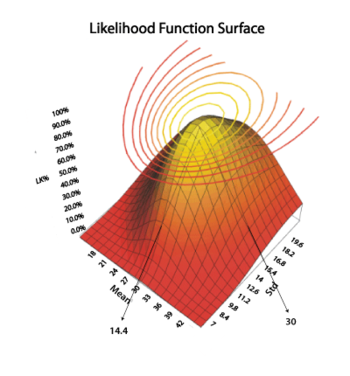
\includegraphics[width=0.5\textwidth]{../Graphics/350px-Apa_fig3}

{\raggedright {\footnotesize Source: \url{reliawiki.org}}}
\end{figure}


If you recall properties of exponents, we can simplify (\ref{eq:8}) as follows:
\begin{align}
\mathcal{L}\left(\mu,\sigma;x_{1},x_{2},\ldots,x_{N}\right)= & \left(\frac{1}{\sqrt{2\pi\sigma^{2}}}\right)^{N}\exp\left(-\frac{\sum_{i=1}^{N}\left(x_{i}-\mu\right)^{2}}{2\sigma^{2}}\right)\nonumber \\
= & \left(\frac{1}{\left(\sqrt{2\pi\sigma^{2}}\right)^{N}}\right)\exp\left(-\frac{\sum_{i=1}^{N}\left(x_{i}-\mu\right)^{2}}{2\sigma^{2}}\right)\label{eq:9}
\end{align}

What does the likelihood function look like? See Figure \ref{fig:mle} for an example where there are two parameters (e.g. $\mu$ and $\sigma^{2}$ in the example above).

\paragraph{The log likelihood function}

Recall that, when ordering a set, one can take a \emph{monotonic transformation} of the set and preserve the ordering. It turns out that we can apply such a transformation to (\ref{eq:9}) by taking the natural logarithm ($\ln$) of both sides. This leaves us with:
\begin{align}
\ln\mathcal{L}\left(\mu,\sigma;x_{1},x_{2},\ldots,x_{N}\right)= & \ln\left[\left(\frac{1}{\left(\sqrt{2\pi\sigma^{2}}\right)^{N}}\right)\exp\left(-\frac{\sum_{i=1}^{N}\left(x_{i}-\mu\right)^{2}}{2\sigma^{2}}\right)\right]\nonumber \\
\ell\left(\mu,\sigma;x_{1},x_{2},\ldots,x_{N}\right)= & \ln\left(\frac{1}{\left(\sqrt{2\pi\sigma^{2}}\right)^{N}}\right)+\ln\left(\exp\left(-\frac{\sum_{i=1}^{N}\left(x_{i}-\mu\right)^{2}}{2\sigma^{2}}\right)\right)\nonumber \\
= & \underbrace{\ln\left(1\right)}_{=0}-\ln\left(\left(2\pi\sigma^{2}\right)^{N/2}\right)-\frac{1}{2\sigma^{2}}\sum_{i=1}^{N}\left(x_{i}-\mu\right)^{2}\nonumber \\
= & -\frac{N}{2}\ln\left(2\pi\sigma^{2}\right)-\frac{1}{2\sigma^{2}}\sum_{i=1}^{N}\left(x_{i}-\mu\right)^{2}\label{eq:10}
\end{align}

Equation (\ref{eq:10}) is known as the \emph{log likelihood function}. Our goal is find the estimated $\mu$ and $\sigma$ that maximize this function.\footnote{Because of monotonicity, the maximum of the likelihood function will be the same as the maximum of the log likelihood function.}

\paragraph{Finding the maximum of the log likelihood function}

To find the maximum likelihood estimates (MLEs) of the log likelihood function, we take the first derivative of $\ell\left(\mu,\sigma;x_{1},\ldots,x_{N}\right)$ with respect to $\mu$ and $\sigma$:
\begin{align}
\frac{\partial}{\partial\mu}\ell\left(\mu,\sigma;x_{1},x_{2},\ldots,x_{N}\right)= & \frac{\partial}{\partial\mu}\left[-\frac{N}{2}\ln\left(2\pi\sigma^{2}\right)-\frac{1}{2\sigma^{2}}\sum_{i=1}^{N}\left(x_{i}-\mu\right)^{2}\right]\nonumber \\
= & -\frac{1}{2\sigma^{2}}\frac{\partial}{\partial\mu}\sum_{i=1}^{N}\left(x_{i}-\mu\right)^{2}\,\,\,\,\ldots\,\,\,\text{(need\,to\,use\,the\,chain\,rule)}\nonumber \\
0= & -\frac{2\cdot\left(-1\right)}{2\sigma^{2}}\sum_{i=1}^{N}\left(x_{i}-\hat{\mu}\right)\label{eq:11}\\
0= & \frac{1}{\sigma^{2}}\left(\sum_{i=1}^{N}x_{i}-N\hat{\mu}\right)\nonumber \\
\hat{\mu}= & \frac{1}{N}\sum_{i=1}^{N}x_{i}\nonumber 
\end{align}

Now with respect to $\sigma^{2}$ (it's easier than with respect to $\sigma$):

\begin{align}
\frac{\partial}{\partial\sigma^{2}}\ell\left(\mu,\sigma;x_{1},x_{2},\ldots,x_{N}\right)= & \frac{\partial}{\partial\sigma^{2}}\left[-\frac{N}{2}\ln\left(2\pi\sigma^{2}\right)-\frac{1}{2\sigma^{2}}\sum_{i=1}^{N}\left(x_{i}-\mu\right)^{2}\right] \nonumber \\
= & \frac{\partial}{\partial\sigma^{2}}\left[-\frac{N}{2}\ln\left(2\pi\right)-\frac{N}{2}\ln\left(\sigma^{2}\right)-\frac{1}{2\sigma^{2}}\sum_{i=1}^{N}\left(x_{i}-\mu\right)^{2}\right] \nonumber \\
= & -\frac{N}{2\sigma^{2}}-\frac{\partial}{\partial\sigma^{2}}\left[\frac{1}{2\sigma^{2}}\sum_{i=1}^{N}\left(x_{i}-\mu\right)^{2}\right] \nonumber \\
0= & -\frac{N}{2\hat{\sigma}^{2}}+\frac{1}{2\left(\hat{\sigma}^{2}\right)^{2}}\sum_{i=1}^{N}\left(x_{i}-\mu\right)^{2}\\
0= & -\frac{N}{2\hat{\sigma}^{2}}+\frac{1}{2\hat{\sigma}^{4}}\sum_{i=1}^{N}\left(x_{i}-\mu\right)^{2} \nonumber \\
0= & \frac{1}{2\hat{\sigma}^{2}}\left[\frac{1}{2\hat{\sigma}^{2}}\sum_{i=1}^{N}\left(x_{i}-\mu\right)^{2}-N\right] \nonumber \\
\hat{\sigma}^{2}= & \frac{1}{N}\sum_{i=1}^{N}\left(x_{i}-\mu\right)^{2} \nonumber
\end{align}
So our Maximum Likelihood Estimate (MLE) is
\begin{align*}
\hat{\mu}= & \frac{1}{N}\sum_{i=1}^{N}x_{i}\\
\hat{\sigma}^{2}= & \frac{1}{N}\sum_{i=1}^{N}\left(x_{i}-\mu\right)^{2}
\end{align*}
and those formulas should look very familiar to you.

\paragraph{Second-order conditions}

For a maximum, we want the second order conditions to be \emph{negative} to ensure that we indeed have a maximum. It turns out that these conditions are satisfied for the MLE of the normal distribution.

\subsection{MLE optimization for linear regression}
Going back to the linear model, let's now assume that $\varepsilon \overset{iid}{\sim}N\left(0,\sigma^2\right)$. We can write down a likelihood function for this model, which is going to look similar to the likelihood function we wrote before, but with a slight tweak---instead of targeting $\mu$ as a parameter, we'll be targeting $\beta$:

\begin{align*}
    \mathcal{L} =& \prod_{i} f\left(\varepsilon_{i}\right) \\
    =& \prod_{i} \frac{1}{\sqrt{2\pi \sigma^{2}}} \exp \left(-\frac{\varepsilon_{i}^{2}}{2\sigma^{2}}\right) \\
    =& \left(\frac{1}{\sqrt{2\pi \sigma^{2}}}\right)^{n} \exp \left(-\frac{\sum_{i}\varepsilon_{i}^{2}}{2\sigma^{2}}\right) \\
    =& \left(\frac{1}{\sqrt{2\pi \sigma^{2}}}\right)^{n} \exp \left(-\frac{\varepsilon^{\prime}\varepsilon}{2\sigma^{2}}\right)\,\,\,,\,\text{and,\,taking\,logs,} \\
    \ell\left(y,X;\beta,\sigma\right)    =& -\frac{n}{2}\ln\left(2\pi\right) - n \ln \left(\sigma\right) - \frac{1}{2\sigma^{2}}\left(y-X\beta\right)^{\prime}\left(y-X\beta\right)
\end{align*}

Our objective is to maximize the likelihood above with respect to $\beta$ and $\sigma$:
\begin{align*}
    & \max_{\beta,\sigma} -\frac{n}{2}\ln\left(2\pi\right) - n \ln \left(\sigma\right) - \frac{1}{2\sigma^{2}}\left(y-X\beta\right)^{\prime}\left(y-X\beta\right) \\
    \frac{\partial\ell}{\partial\beta} =& \frac{1}{2\sigma^{2}}\frac{\partial}{\partial\beta}\left(y-X\beta\right)^{\prime}\left(y-X\beta\right) \\
    0 =& \frac{1}{2\sigma^{2}}\left[-2X^{\prime}y +2\left(X^{\prime}X\right)\hat{\beta}\right] \\
    \hat{\beta} =& \left(X^{\prime}X\right)^{-1}X^{\prime}y \\
    \frac{\partial\ell}{\partial\sigma} =& -\frac{n}{\sigma} + \frac{\left(y-X\beta\right)^{\prime}\left(y-X\beta\right)}{\sigma^{3}} \\
    0 =& -\frac{n}{\hat{\sigma}} +  \frac{\left(y-X\beta\right)^{\prime}\left(y-X\beta\right)}{\hat{\sigma}^{3}} \\
    \frac{n}{\hat{\sigma}} =& \frac{\left(y-X\beta\right)^{\prime}\left(y-X\beta\right)}{\hat{\sigma}^{3}} \\
    \hat{\sigma}^{2} =& \frac{\left(y-X\beta\right)^{\prime}\left(y-X\beta\right)}{n} 
\end{align*}

Second-order conditions for a maximum require that the matrix below be \emph{negative definite}\footnote{Negative definite is how we tell that a matrix is ``negative.''}:

\begin{align}
    \label{eq:hess}
    \left[ {\begin{array}{cc}
                \frac{\partial^{2}\ell}{\partial\beta\partial\beta^{\prime}} & \frac{\partial^{2}\ell}{\partial\beta\partial\sigma}  \\
                \frac{\partial^{2}\ell}{\partial\sigma\partial\beta^{\prime}} & \frac{\partial^{2}\ell}{\partial\sigma^{2}}  \\
                  \end{array} } \right]
                  =&
    \left[ {\begin{array}{cc}
                - \frac{X^{\prime}X}{\hat{\sigma}^{2}} &  \frac{X^{\prime}X\hat{\beta} - X^{\prime}y}{\hat{\sigma}^{3}}  \\
                \frac{\hat{\beta}^{\prime}X^{\prime}X - y^{\prime}X}{\hat{\sigma}^{3}}  & \frac{n}{\hat{\sigma}^{2}} - \frac{3\left(y-X\hat{\beta}\right)^{\prime}\left(y-X\hat{\beta}\right)}{\hat{\sigma}^{4}}  \\
                  \end{array} } \right]
              \end{align}


\subsection{Vocabulary}
\begin{description}
    \item[closed-form~solution] A solution to an optimization problem that can be expressed as a mathematical formula. For example, $\hat{\beta} = \left(X^{\prime}X\right)^{-1}X^{\prime}y$ is a closed-form solution to the parameters of the classical linear model. This solution holds for either ordinary least squares (OLS) minimization or maximum likelihood estimaiton (MLE)

        Most optimization problems do \emph{not} have a closed-form solution, in which case we will need a computer to iteratively ``guess and check'' different candidate parameters to find the minimum or maximum of our objective function.

        We will talk about these in the next couple of classes.

    \item[gradient~vector] The gradient vector is the vector of first derivatives of the objective function. For MLE problems, it is the vector
 
        \begin{align*}
    \left[ {\begin{array}{c}
                \frac{\partial\ell}{\partial\beta}  \\
                \frac{\partial\ell}{\partial\sigma} \\
                  \end{array} } \right]
                  =&
    \left[ {\begin{array}{c}
\frac{1}{2\sigma^{2}}\left[-2X^{\prime}y +2\left(X^{\prime}X\right)\hat{\beta}\right] \\
-\frac{n}{\hat{\sigma}} +  \frac{\left(y-X\beta\right)^{\prime}\left(y-X\beta\right)}{\hat{\sigma}^{3}} \\
                  \end{array} } \right]
        \end{align*}

\item[hessian~matrix] The hessian matrix is the matrix of second derivatives of the objective function. For MLE problems, it is the matrix listed in \eqref{eq:hess}.

\end{description}

Why do we need to know these three vocabulary words? Because we need to understand how the computer finds the optimum of our objective function. For the 99\% of problems that don't have a closed-form solution, the computer tries to find the values of the parameters that set the gradient vector equal to zero. Depending on the algorithm, it will also check that the hessian matrix is negative definite (if we are maximizing) or positive definite (if we are minimizing). 

\section{Math: logistic regression}
The above examples optimized the classical linear model, which is a model where the dependent variable is continuous and the optimization has a closed-form solution.

Now let's look at a case where the dependent variable $y$ is binary and (without loss of generality) takes on values 0 and 1.

The appropriate statistical distribution to model a 0/1 outcome is known as the \emph{Bernoulli distribution}. In this distribution, $y=1$ with probability $p$ and $y=0$ with probability $1-p$. You can think of a Bernoulli distribution as modeling a weighted coin flip, where heads occurs with probabiliy $p$.

The probability density function (pdf) of the Bernoulli distribution is
\[
    f\left(y;p\right) = p^{y}\left(1-p\right)^{1-y}
\]

Now let's return to our classical linear model, but where $y$ is now binary instead of continuous. As before, we have (in matrix form)
\[
y = X\beta + \varepsilon
\]

Now we want to think about the conditions under which $y=1$ (which occurs with probability $p$).
\begin{align*}
    \Pr\left(y=1\right) =& \Pr\left(y>0\right) \\
                        =& \Pr\left(X\beta + \varepsilon > 0\right) \\
                        =& \Pr\left(X\beta > -\varepsilon \right) \\
                        =& \Pr\left(-\varepsilon < X\beta \right) \\
    =& \Pr\left(\varepsilon < X\beta \right)\,\,\,\text{if}\,\,\varepsilon\,\,\text{has\,a\,symmetric\,distribution} \\
    =& F\left(X\beta\right)
\end{align*}
where $F\left(\cdot\right)$ denotes the cumulative distribution function of $\varepsilon$.

\subsection{MLE of the logistic regression model}
If we assume that $\varepsilon$ is drawn from the logistic distribution (instead of the normal distribution as in \eqref{eq:8}), then we get
\begin{align*}
    F\left(x\right) =& \frac{1}{1+e^{-x}} \\
                    =& \frac{e^{x}}{1+e^{x}} \\
\end{align*}

This is known as the \textbf{logistic probability function}, or the \textbf{sigmoid function}.

If we go back to the previous set of equations and think about our Bernoulli parameter $p$, we have that $p=\Pr\left(y=1\right)=F\left(X\beta\right)=\frac{\exp\left(X\beta\right)}{1+\exp\left(X\beta\right)}$.

\subsubsection{Logit likelihood function}
Combining the above results, we get our likelihood function:
\begin{align}
    \label{eq:logit}
    \mathcal{L}\left(y,X;\beta\right) =& \prod_{i}p_{i}^{y_{i}}\left(1-p_{i}\right)^{1-y_{i}} \nonumber \\
                                      =& \prod_{i}\left(\frac{\exp\left(X\beta\right)}{1+\exp\left(X\beta\right)}\right)^{y_{i}}\left(1-\frac{\exp\left(X\beta\right)}{1+\exp\left(X\beta\right)}\right)^{1-y_{i}} \nonumber \\
                                      =& \prod_{i}\left(\frac{\exp\left(X\beta\right)}{1+\exp\left(X\beta\right)}\right)^{y_{i}}\left(\frac{1}{1+\exp\left(X\beta\right)}\right)^{1-y_{i}} \nonumber \\
    \ell\left(y,X;\beta\right) =& \sum_{i}y_{i}\ln\left(\frac{\exp\left(X\beta\right)}{1+\exp\left(X\beta\right)}\right)+\left(1-y_{i}\right)\ln\left(\frac{1}{1+\exp\left(X\beta\right)}\right) 
\end{align}

\subsubsection{Logit first order conditions}
The first order conditions of \eqref{eq:logit} are:
\begin{align}
    \label{eq:logitFOC}
    \frac{\partial\ell}{\partial\beta} =& \frac{\partial\ell}{\partial\beta}y\left[X\beta - \ln\left(1+\exp\left(X\beta\right)\right)\right] - \left(1-y\right)\left[\ln\left(1+\exp\left(X\beta\right)\right)\right] \nonumber \\
0 =& \frac{\partial\ell}{\partial\beta}y\left[X\beta\right] - \ln\left(1+\exp\left(X\beta\right)\right) \nonumber \\
    0 =& X^{\prime}y-\left[\frac{1}{1+\exp\left(X\beta\right)}X\exp\left(X\beta\right)\right] \nonumber \\
    0 =& X^{\prime}y-\left[X\frac{\exp\left(X\beta\right)}{1+\exp\left(X\beta\right)}\right] \nonumber \\
    0 =& X^{\prime}y-X^{\prime}p \nonumber \\
    0 =& X^{\prime}\left(y-p\right) \nonumber \\
    0 =& X^{\prime}\left(y-\frac{\exp\left(X\beta\right)}{1+\exp\left(X\beta\right)}\right) 
\end{align}

Now we need to solve for $\beta$:
\[
    X^{\prime}y=X^{\prime}\left(\frac{\exp\left(X\beta\right)}{1+\exp\left(X\beta\right)}\right)
\]
But this does not have a closed-form solution! Hence, we need to use numerical methods such as gradient descent or L-BFGS to iteratively ``guess and check'' various values of the $\beta$ vector that solve \eqref{eq:logitFOC}.

\end{document}

